
\documentclass[twoside,10.5pt]{article}%                         
\usepackage{mathrsfs}%                                           
\usepackage{pifont}%                                             
\usepackage{amsmath}%                                            
\usepackage{amsthm}%                                             
\usepackage{txfonts}%                                            
\usepackage{geometry}%                                           
\usepackage{latexsym}%                                           
\usepackage{amssymb}%                                            
\usepackage{graphicx}%                                           
\usepackage{geometry}%                                           
\usepackage{xcolor} %                                            
\geometry{paperheight=28.5cm,paperwidth=21cm,top=2.5cm,%         
bottom=2.6cm,left=2.5cm,right=2.5cm,headheight=0.8cm,%             
headsep=0.9cm,textheight=20cm,footskip=1cm}%                   
\setlength{\parindent}{0pt} \setlength{\parskip}{5pt}%           
\renewcommand{\baselinestretch}{1.0}%                            *                                                        *
\pagestyle{empty}
\begin{document}

\begin{center}
{\LARGE{Algoritmos de Ordenaci\'on}}\\[20pt]
\end{center}

\textbf{1. Introducci\'on}

\emph{1.1 Algoritmos de Ordenaci\'on}
En computaci\'on y matem\'aticas un {\color{blue} algoritmo de ordenamiento} es un algoritmo que pone elementos de una lista o un vector en una secuencia dada por una relaci\'on de orden, es decir, el resultado de salida ha de ser una permutaci\'on —o reordenamiento— de la entrada que satisfaga la relaci\'on de orden dada. Las relaciones de orden m\'as usadas son el orden num\'erico y el orden lexicogr\'afico (Wikipedia). En esta primera parte mostraremos algunos algoritmos b\'asicos de ordenaci\'on, codificados en Python.

\textbf{2. Algoritmos}




\emph{2.1 Ordenamiento de burbuja (Bubble Sort)}


\emph{2.2 Ordenamiento por inserci\'on (Insertion Sort) }


\emph{2.3 Ordenamiento por mezcla (Merge Sort)}

\emph{2.4 Ordenamiento r\'apido   (QuickSort)}

\emph{2.5 Ordenamiento por selecci\'on (Selection Sort)}

\emph{2.6 Ordenamiento shell  (Shell Sort)}



\textbf{3. Explicaciones}

\emph{3.1 Ordenamiento de burbuja (Bubble Sort)}
El m\'etodo de la burbuja es uno de los mas simples algoritmos de ordenaci\'on, es  como comparar todos
los elementos de una lista contra todos, si se cumple que uno es mayor o menor a
otro, entonces se  intercambia de posici\'on.

\begin{figure}[h]
  \centering
  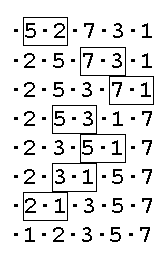
\includegraphics[scale=.5]{burbuja.png}
  \caption{Ordenamiento de burbuja.} 
 \end{figure}


\emph{3.2 Ordenamiento por inserci\'on (Insertion Sort)}
Este m\'etodo tiene la semejanza con la forma de clasificar las cartas de una baraja, insertando cada carta en el lugar adecuado. El algoritmo ordena los dos primeros elementos de la lista, a continuaci\'on el tercer elemento se inserta en la posici\'on que corresponda, el cuarto se inserta en la lista de tres elementos, y as\'i sucesivamente. Este proceso continua hasta que la lista este totalmente ordenada.

\begin{figure}[h]
   \centering
   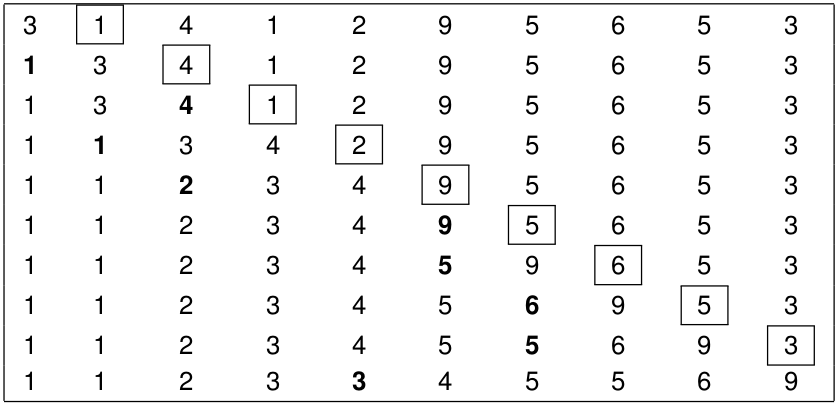
\includegraphics[scale=.35]{insercion.png}
   \caption{Ordenamiento por inserci\'on.} 
  \end{figure}

\emph{3.3 Ordenamiento por selecci\'on (Selection Sort)}
(Wikipedia) Es un algoritmo de ordenaci\'on que funciona de la siguiente manera:

\begin{itemize}
\item Busca el m\'inimo elemento entre una posici\'on i y el final de la lista.
\item Intercambiar el m\'inimo con el elemento de la posici\'on i.
\end{itemize}

Por ejemplo,se recorre una lista, se selecciona el elemento menor y se intercambia este elemento con el de la primera posici\'on. 

\begin{figure}[h]
   \centering
   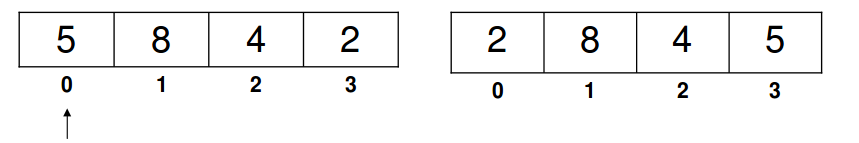
\includegraphics[scale=.35]{selec1.png}
   %\caption{Ordenamiento por seleccion.} 
  \end{figure}

Se hace lo mismo, pero ahora se busca desde la segunda posici\'on hasta el final el menor. Se intercambia \'este menor con lo que est\'a en la segunda posici\'on.

\begin{figure}[h]
   \centering
   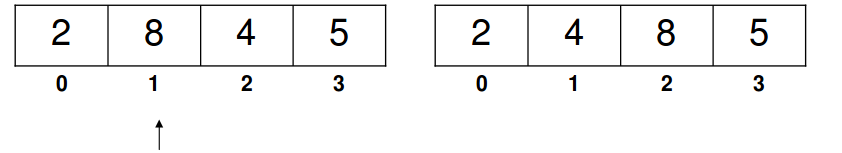
\includegraphics[scale=.35]{selec2.png}
   %\caption{Ordenamiento por seleccion.} 
  \end{figure}

Se repite para las siguientes posiciones, hasta la posici\'on $n-1$, si es que la lista  tiene longitud $n$.

\begin{figure}[h]
    \centering
    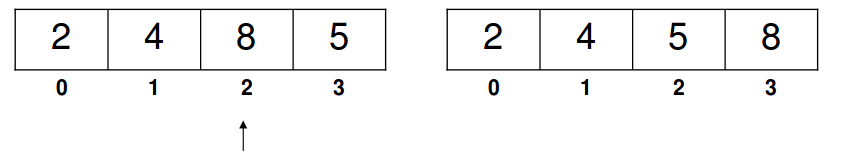
\includegraphics[scale=.35]{selec3.png}
    %\caption{Ordenamiento por seleccion.} 
   \end{figure}
 

\emph{3.4 Ordenamiento por mezcla (Merge Sort)}
El algoritmo de ordenamiento por mezcla (Merge Sort) es un algoritmo de ordenamiento  basado en la {\color{red}t\'ecnica divide y vencer\'as}, desarrollado por John Von Neumann.

(Wikipedia) El ordenamiento por mezcla funciona de la siguiente manera:
\begin{itemize}
\item Si la longitud de la lista es 0 \'o 1, entonces ya est\'a ordenada. En otro caso:
\item Dividir la lista desordenada en dos sublistas de aproximadamente la mitad del tama\~no.
\item Ordenar cada sublista recursivamente aplicando el ordenamiento por mezcla.
\item Mezclar las dos sublistas en una sola lista ordenada.
\end{itemize}

Si se piensa en este algoritmo recursivamente, podemos imaginar que dividir\'a la lista
hasta tener un elemento en cada lista, luego lo compara con el que est\'a a su lado y
seg\'un corresponda, lo situa donde corresponde. En la figura se ve como funciona.

\begin{figure}[h]
   \centering
   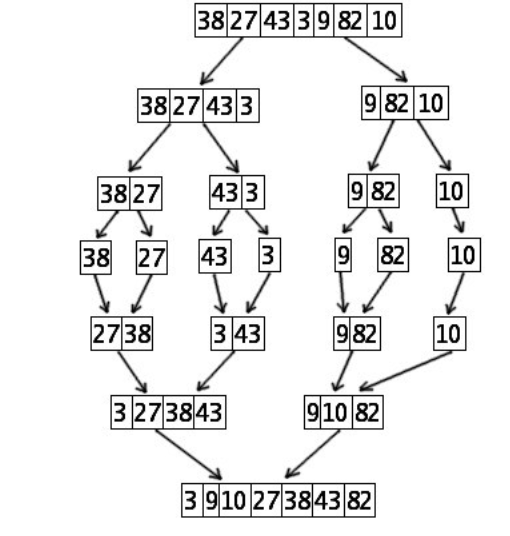
\includegraphics[scale=.35]{merge.png}
   \caption{Ordenamiento por mezcla.} 
  \end{figure}

\emph{3.5   Ordenamiento r\'apido   (QuickSort)}
(Wikipedia) El ordenamiento r\'apido (quicksort) es un algoritmo  basado en la t\'ecnica de divide y vencer\'as, que permite, en promedio, ordenar $n$ elementos en un tiempo proporcional a $n\log n$.

El algoritmo trabaja de la siguiente forma:

\begin{itemize}
\item Elegimos un elemento de la lista de elementos a ordenar, al que llamaremos pivote.
\item Acomodamos  los dem\'as elementos de la lista a cada lado del pivote, de manera que a un lado queden todos los menores que \'el, y al otro los mayores. Los elementos iguales al pivote pueden ser colocados tanto a su derecha como a su izquierda, dependiendo de la implementaci\'on deseada. En este momento, el pivote ocupa exactamente el lugar que le corresponderá en la lista ordenada.
\item La lista queda separada en dos sublistas, una formada por los elementos a la izquierda del pivote, y otra por los elementos a su derecha.
\item Repetimos este proceso de forma recursiva para cada sublista mientras \'estas contengan m\'as de un elemento. Una vez terminado este proceso todos los elementos estar\'an ordenados.
\end{itemize}

La eficiencia del algoritmo depende de la posici\'on en la que termine el pivote elegido. La siguiente figura muestra de mejor manera lo mencionado, usando como pivote el primer elemento.


\begin{figure}[h]
   \centering
   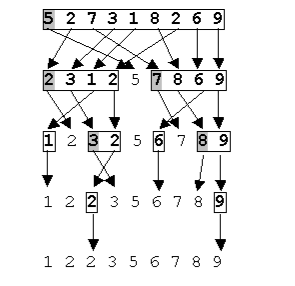
\includegraphics[scale=.65]{quicksort.png}
   \caption{Ordenamiento r\'apido (quicksort).} 
  \end{figure}

\newpage


\emph{3.6   Ordenamiento shell  (Shell Sort)}
Es un algoritmo de ordenaci\'on muy ingenioso, basado en comparaciones e intercambios. (Ecured) el algoritmo Shell es una mejora de la ordenaci\'on por inserci\'on, donde se van comparando elementos distantes, al tiempo que se los intercambian si corresponde. A medida que se aumentan los pasos, el tama\~no de los saltos disminuye; por esto mismo, es \'util tanto como si los datos desordenados se encuentran cercanos, o lejanos.

Es bastante adecuado para ordenar listas de tama\~no moderado, debido a que su velocidad es aceptable y su codificaci\'on es  sencilla. 

\end{document}
